%
% chapter.tex -- Kapitel über Spline Wavelets
%
% (c) 2019 Prof Dr Andreas Müller, Hochschule Rapperswil
%
\chapter{Spline-Wavelets
\label{chapter:spline}}
\lhead{Spline-Wavelets}
\rhead{}
Das Haar-Wavelet ist charakterisiert durch die erzeugende Funktion $H_0$,
die in einer Funktionalgleichung der Fourier-Transformierten von $\varphi$
vorkommt.
Es stellt sich heraus, dass sich eine solche Funktionalgleichung für 
Faltungen von $\varphi$ mit sich selbst sofort ableiten lassen.
Allerdings bilden die verschobenen Kopien keine orthonormierte Basis,
dazu müssen sie erst orthonormiert werden.
Da sich dafür aber ein Verfahren angeben lässt, kann man eine Familie 
von Wavelets konstruieren, die sich dadurch auszeichnen, dass sie
stückweise polynomiell sind, genauso wie das Haar-Wavelet stückweise
konstant war.
Dies sind die B-Spline-Wavelets, die in diesem Kapitel dargestellt werden
sollen.

Die B-Spline-Wavelets haben nicht kompakten Träger, aber Koeffizienten
mit grossem Index sind sehr klein.
Ausserdem sind sie wie die Wavelet-Koeffizienten typischerweise irrational,
müssen also in einer Implementation notwendigerweise gerundet werden.
Die Stabilität der Wavelet-Transformation stellt sicher, dass die Rundung
nicht zu unbrauchbaren Resultaten führt.
Indem sehr kleine Koeffizienten zu $0$ gerundet werden, können auch die
B-Spline-Wavelets als Wavelets mit kompaktem Träger behandelt werden.
Dasselbe gilt natürlich auch für jede andere Form von Wavelet, bei dem
die Werte der Koeffizienten rasch gegen $0$ gehen.

%
% faltung.tex
%
% (c) 2019 Prof Dr Andreas Müller, Hochschule Rapperswil
%
\section{Faltung
\label{section:faltung}}
\rhead{Faltung}
Die Faltung kann dazu verwendet werden, neue Funktionen zu erzeugen.
Dazu müssen wir verstehen, wie die Faltung und die Operatoren $T_b$ und
$D_b$ zusammenwirken.
Wir erinnern an die Definition~\ref{definition:faltung} und die
Formel \eqref{definition:formel:faltung}
\[
(f*g)(t)
=
\int_{-\infty}^\infty f(s)g(t-s)\,ds
\]
für die Faltung.

\subsection{Faltung als Skalarprodukt}
\index{Faltung als Skalarprodukt}%
Die Faltung ist ein Integral über ein Produkt von Funktionen,
kann man sie als Skalarprodukt schreiben?
Leider hat die Integrationsvariable im Faktor $g(t-s)$ das falsche
Vorzeichen, die Funktion ist ``verkehrt''.
Wir korrigieren dies mit Hilfe des Umkehroperators, der wie folgt
definiert ist.

\begin{definition}
Der Operator $R$ wirkt auf eine Funktion $f(t)$ mittels
\[
(Rf)(t) = f(-t).
\]
$R$ heisst {\em Umkehrungsoperator} (engl.~{\em Reversing operator}).
\end{definition}
\index{Umkehrungsoperator}%
\index{Reversing oeprator}%

Offenbar ist $R$ eine Isometrie von $L^2(\mathbb R)$.
$R$ ist ein Spezialfall des Skalierungsoperators: $R=D_{-1}$.
Daraus ergeben sich automatisch die Rechenregeln
\[
T_aR = RT_a = T_{-a}
\qquad\text{und}\qquad
D_aR = D_{-a}=RD_a.
\]

Mit Hilfe des Operators $R$ lässt sich die Faltung jetzt als
Skalarprodukt schreiben.
Es ist nämlich
\begin{align*}
(f*g)(t)
&=
\int_{-\infty}^\infty f(s) g(t-s) \,ds
=
\int_{-\infty}^\infty f(s) (Rg)(s-t) \,ds
=
\int_{-\infty}^\infty f(s) (T_tRg)(s) \,ds
=
\langle f,T_tRg\rangle.
\end{align*}
Mit dieser Schreibweise lässt sich das Zusammenspiel zwischen Faltung
und den Operatoren $T_b$ und $D_a$ viel leicht verstehen.

\subsection{Faltung und Translation und Dilatation
\label{subsection:translation-und-dialatation}}
Mit Hilfe der Darstellung als Skalarprodukt können wir jetzt sofort
die Faltung von translierten oder skalierten Funktionen ermitteln.

Wir beginnen mit der Faltung der Translate $T_bf$ und $T_cg$:
\begin{align*}
(T_bf * T_cg)(t)
&=
\langle T_bf, T_tRT_cg\rangle
=
\langle T_bf, T_tT_{-c}Rg\rangle
=
\langle f, T_{-b}T_tT_{-c}Rg\rangle
\\
&=
\langle f, T_{-b+t-c}Rg\rangle
=
T_{b+c}
\langle f, T_tRg\rangle
=
T_{b+c}(f*g)(t).
\end{align*}
Wir formulieren dieses Resultat als

\begin{satz}
Für beliebige Funktionen $f,g\in L^2(\mathbb R)$ gilt
\begin{equation}
T_bf*T_cg
=
T_{b+c}(f*g).
\label{eq:Tconv}
\end{equation}
\end{satz}

In ganz ähnlicher Weise können wir auch die Faltung von
$D_af$ und $D_ag$ bestimmen:
\begin{align*}
(D_af * D_ag)(t)
&=
\langle D_af, T_tRD_ag\rangle
=
\langle D_af, T_tD_aRg\rangle
=
\langle D_af, D_aT_{t/a}Rg\rangle
\\
&=
\langle f, T_{t/a}Rg\rangle
=
\sqrt{a} D_a \langle f, T_t Rg\rangle
=
\sqrt{a}(D_a (f*g))(t).
\end{align*}
In der Skalierungsrelation einer Multiskalenanalyse kommen keine
gemischten Skalierungsfaktoren $a$ vor, daher reicht die Form
\eqref{eq:Dconv} für die nachfolgenden Rechnung aus.
Für gemischte Skalierungsfaktoren lässt sich keine Formel angeben,
wie in Übungsaufgabe~1 dieses Kapitels gezeigt wird.

\begin{satz}
\label{satz:faltung:Da}
Für beliebige Funktionen $f,g\in L^2(\mathbb R)$ gilt
\begin{align}
D_af * D_ag &= \sqrt{a}D_a(f*g)
&&\text{und}
&
\tilde{D}_af * \tilde{D}_ag &= a\tilde{D}_a(f*g).
\label{eq:Dconv}
\end{align}
für $a>0$.
\end{satz}

\begin{proof}[Beweis]
Wir müssen nur noch die zweite Formel für den Operator $\tilde{D}_a$
nachweisen.
Dazu verwenden wir die Relation $D_af = \sqrt{a}\tilde{D}_a$ und die
erste Beziehung in \eqref{eq:Dconv} und erhalten
\[
\tilde{D}_af * \tilde{D}_ag
=
\sqrt{a}D_af * \sqrt{a}D_ag
=
a
\sqrt{a}
D_a (f*g)
=
a
\tilde{D}_a(f*g).
\]
Damit ist auch die zweite Relation bewiesen.
\end{proof}


\subsection{Linearkombinationen
\label{subsection:linearkombinationen}}
Ein wesentlicher Aspekt einer Multiskalenanalyse ist, dass das
Vaterwavelet $\varphi$ eine Linearkombination von skalierten
Translaten $D_{\frac12}T_k\varphi$ des Vater-Wavelets ist.
Wir vereinfachen die manchmal etwas umständlichen Formeln für
die Skalierungsrelationen etwas, indem wir auf beiden Seiten
den Operator $D_2$ anwenden.
Dies führt auf die folgende Definition.

\begin{definition}
Wir sagen, eine Funktion $f$ erfüllt die {\em Skalierungseigenschaft},
wenn es Koeffizienten $f_k$ gibt derart, dass
\[
D_2f = \sum_{k\in\mathbb Z} f_k T_kf
\]
\end{definition}

\begin{satz}
\label{satz:faltung-linearkombination}
Sind $f$ und $g$ Funktionen, die beide die Skalierungseigenschaft
mit Koeffizienten $f_k$ und $g_l$
haben, dann hat auch $h=f*g$ die Skalierungseigenschaft
mit Koeffizienten
\begin{equation}
h_s = \frac1{\sqrt{2}} \sum_{k+l=s}f_kg_l.
\label{eq:faltung-linearkombination}
\end{equation}
\end{satz}

\begin{proof}[Beweis]
Seien $f_k$ und $g_k$ die Koeffizienten der Skalierungsrelation von $f$
bzw.~$g$, also
\begin{align*}
D_2f
&=
\sum_{k\in\mathbb Z} f_k T_kf
&
D_2g
&=
\sum_{k\in\mathbb Z} g_k T_kg.
\end{align*}
Nach \eqref{eq:Dconv} ist die Faltung der Funktionen $D_2f$ und $D_2g$
\[
D_2f * D_2g
=
\sqrt{2}
D_2(f*g)
=
\sqrt{2}
D_2h.
\]
Andererseits können wir auch die Faltung der Linearkombinationen 
berechnen:
\begin{align*}
D_2f * D_2g
&=
\biggl( \sum_{k\in\mathbb Z} f_kT_kf \biggr)
*
\biggl( \sum_{l\in\mathbb Z} g_lT_lg \biggr)
\\
&=
\sum_{s\in\mathbb Z}
\sum_{k+l=s} f_kg_l T_kf * T_lg
=
\sum_{s\in\mathbb Z}
\sum_{k+l=s} f_kg_l T_{k+l}(f * g)
=
\sum_{s\in\mathbb Z}
\biggl(\sum_{k+l=s} f_kg_l\biggr) T_sh
\end{align*}
Es folgt, dass
\[
D_2h
=
\frac1{\sqrt{2}} D_2f * D_2g
=
\sum_{s\in\mathbb Z}
\biggl(\frac1{\sqrt{2}}\sum_{k+l=s} f_kg_l\biggr) T_sh.
\]
Dies ist eine Skalierungsrelation für die Funktion $h$, die Koeffizienten
sind
\[
h_s = \frac1{\sqrt{2}} \sum_{k+l=s}f_kg_l.
\]
Damit ist alles bewiesen.
\end{proof}

\subsection{Faltung im Frequenzbereich
\label{subsection:faltung-im-frequenzbereich}}
Wir können dieses Resultat auch im Frequenzbereich formulieren.
Wir haben im Abschnitt~\ref{section:skalfour} die Skalierungsrelation
für die Fourier-Transformierte $\hat{\varphi}$ von $\varphi$ mit Hilfe
der erzeugenden Funktion
\[
H(\omega)
=
\frac{1}{\sqrt{2}}
\sum_{k\in\mathbb Z} h_ke^{ik\omega}
\]
(siehe Definition~\ref{definition:erzeugende-funktion-msa})
als
\begin{equation}
\hat{\varphi}(\omega)
=
H\biggl(\frac{\omega}2\biggr)
\,
\hat{\varphi}\biggl(\frac{\omega}2\biggr)
\label{faltung:skalierung}
\end{equation}
geschrieben.
Sind
$(\varphi_1,H_1)$ und $(\varphi_2,H_2)$ zwei Paare von Funktionen,
welche beide die Skalierungsrelation~\eqref{faltung:skalierung} erfüllen,
dann folgt
\begin{align*}
%\hat{\varphi}_1(\omega)
%&=
%H_1\biggl(\frac{\omega}2\biggr)
%\hat{\varphi}_1 \biggl(\frac{\omega}2\biggr)
%&&\wedge&
%\hat{\varphi}_1(\omega)
%=
%H_1\biggl(\frac{\omega}2\biggr)
%\hat{\varphi}_1\biggl(\frac{\omega}2\biggr)
%&&\Rightarrow&
\hat{\varphi}_1(\omega)
\cdot
\hat{\varphi}_2(\omega)
&=
H_1\biggl(\frac{\omega}2\biggr)
\cdot
H_2\biggl(\frac{\omega}2\biggr)
\cdot
\hat{\varphi}_1\biggl(\frac{\omega}2\biggr)
\cdot
\hat{\varphi}_2\biggl(\frac{\omega}2\biggr)
\\
%&&&&
%&\Rightarrow&
\Rightarrow\qquad
\widehat{\mathstrut\varphi_1*\varphi_2}(\omega)
&=
H_1\biggl(\frac{\omega}2\biggr)
H_2\biggl(\frac{\omega}2\biggr)
\,
\widehat{\mathstrut\varphi_1*\varphi_2}\biggl(\frac{\omega}2\biggr).
\end{align*}
In der zweiten Zeile haben wir den gemeinsamen Faktor $\sqrt{2\pi}$
auf beiden Seiten weggelassen.
Die Faltung $\varphi_1*\varphi_2$ erfüllt also die Skalierungsrelation
mit der erzeugenden Funktion $H_1\cdot H_2$, die wegen
\[
H_1(\omega)\,H_2(\omega)
=
\frac{1}{\sqrt{2}}
\sum_{k\in\mathbb Z} h_{1,k}e^{ik\omega}
\cdot
\frac{1}{\sqrt{2}}
\sum_{l\in\mathbb Z} h_{2,l}e^{il\omega}
=
\frac{1}{\sqrt{2}}
\sum_{s\in\mathbb Z} e^{is\omega}
\frac{1}{\sqrt{2}}
\sum_{k+l=s}h_{1,k}h_{2,l}
\]
die Koeffizienten
\[
h_s = \frac{1}{\sqrt{2}}\sum_{k+l=s} h_{1,k}h_{2,l}
\]
hat,
wie bereits im Satz~\ref{satz:faltung-linearkombination} gezeigt worden ist.


%
% splines.tex
%
% (c) 2019 Prof Dr Andreas Müller, Hochschule Rapperswil
%
\section{Spline-Funktionen
\label{section:spline-funktionen}}
In diesem Abschnitt konstruieren wir ausgehend vom Haar-Wavelet mit Hilfe
der Faltung eine Familie $\varphi^{(n)}$ von Funktionen die zunehmend glatt
sind in dem Sinne, dass $\varphi^{(n)}$ für $n>1$ $n$ mal stetig
differenzierbar ist, und die alle eine Skalierungsrelation erfüllen.
Diese Funktionen werden wir dann im nächsten Abschnitt jeweils ein
Wavelet konstruieren.

\subsection{Das Haar-Wavelet
\label{subsection:spline:haar}}
Das Vater-Wavelet des Haar-Wavelets war die charakteristische Funktion
des Einheitsintervals
\begin{equation}
\varphi^{(0)}(t)
=
\chi_{[0,1)}(t)
=
\begin{cases}
1\qquad\qquad&0\le t < 1\\
0\qquad\qquad&\text{sonst}.
\end{cases}
\end{equation}
Aus $\varphi^{(0)}$ lässt sich wie in Kapitel~\ref{chapter:haar-wavelet}
ausgeführt in eine Multiskalen-Analyse verwandeln.
Eine solche garantiert zunächst einmal eine lineare Darstellung von
$\varphi^{(0)}$ duch skalierte und translierte Kopien von $\varphi^{(0)}$
in der Form
\begin{equation}
\varphi^{(0)}(t)
=
\sqrt{2}
\sum_{k\in\mathbb Z}
h_k\varphi(2t-k)
=
\sum_{k\in\mathbb Z}
h_k D_{\frac12}T_k\varphi^{(0)}(t).
\label{splines:skalierungsrelation}
\end{equation}
Aus der Skalierungsrelation~\eqref{splines:skalierungsrelation}
kann man dann das Mutter-Wavelet gewinnen, wie in
Abschnitt~\ref{section:mutter-aus-vater} gezeigt wird.
Im Falle des Haar-Wavelets sind sind die Koeffzienten der
Skalierungsrelation
\[
\varphi^{(0)}(t)
=
\sqrt{2}
\biggl(
\frac1{\sqrt{2}}
\varphi^{(0)}(2t)
+
\frac1{\sqrt{2}}
\varphi^{(0)}(2t-1)
\biggr)
\qquad
\Rightarrow
\quad
h_0 = h_1 = \frac{1}{\sqrt{2}}.
\]
Nach Lemma~\ref{lemma:msa:psirelation} ist dann das Mutterwavelet
\[
\psi^{(0)}(t)
=
\sqrt{2}
\biggl(
\frac{1}{\sqrt{2}}
\varphi^{(0)}(2t)
-
\frac{1}{\sqrt{2}}
\varphi^{(0)}(2t-1)
\biggr),
\]
wie ebenfalss bereits in Kapitel~\ref{chapter:haar-wavelet}.
Auch wurde bereits auf die schlechten Stetikeitseigenschaften und
die schlechte Frequenz-Lokalisierung des Haar-Wavelets hingewiesen,
welche den praktischen Nutzen des Haar-Wavelets limitiert.
Damit stellt sich das Problem, ob man Funktionen gewinnen kann, die
eine ähnlich einfach zu gewinnende Skalierungsrelation haben.

\subsection{Splines
\label{subsection:splines}}
Gesucht ist jetzt also eine Vater-Wavelet-Funktion, welche ähnlich
einfach ist wie das eben repetiert Haar-Wavelet, aber bessere 
Stetigkeitseigenschaften und damit bessere Lokalisierung im Frequenzbereich
hat.

Wir definieren die Funktionen $\varphi^{(n)}$ rekursiv wie folgt.

\begin{definition}
Die Funktion $\varphi^{(0)}$ ist wie vorhin die charakteristische Funktion
des Einheitsintervals.
Für $n>0$ setzt man
\[
\varphi^{(n)} = \varphi^{(0)} * \varphi^{(n-1)}.
\]
\end{definition}

Man beachte, dass die Funktionen $\varphi^{(n)}$ zwar in $L^2(\mathbb R)$ 
sind, aber sie sind nicht normiert.
Erst recht sind die Translate nicht orthonormiert, wie man das für eine
Multiskalenanalyse erwarten würde.

Explizit bedeutet die Definition der Funktion $\varphi^{(n)}$
\begin{equation}
\varphi^{(n)}(t)
=
\int_{-\infty}^\infty
\varphi^{(0)}(s)
\varphi^{(n-1)}(t-s)
\,ds
=
\int_0^1
\varphi^{(n-1)}(t-s)
\,ds
=
-
\int_t^{t-1}
\varphi^{(n-1)}(\tau)
\,d\tau
=
\int_{t-1}^t \varphi^{(n-1)}(\tau)\,d\tau
\label{eq:varphin-berechnung}
\end{equation}
mit der Substitution $\tau=t-s$.

\begin{lemma}
\label{lemma:phidiffbar}
Die Funktion $\varphi^{(n)}$ ist für $n>1$ $n$ mal stetig differenzierbar.
\end{lemma}

\begin{proof}[Beweis]
Mit Hilfe der Formel~\eqref{eq:varphin-berechnung} kann man die Ableitung
\begin{align*}
\frac{d}{dt}
\varphi^{(n)}(t)
&=
\frac{d}{dt} \int_{t-1}^t \varphi^{(n-1)}(\tau)\,d\tau
=
\varphi^{(n-1)}(\tau)\bigg|_{\tau=t}
-
\varphi^{(n-1)}(\tau)\bigg|_{\tau=t-1}
=
\varphi^{(n-1)}(t)-\varphi^{(n-1)}(t-1)
\end{align*}
berechnen.
Für $n>1$ ist die Funktion $\varphi^{(n-1)}$ stetig, also auch die
Ableitung.
Damit ist $\varphi^{(n)}$ stetig differenzierbar.
\end{proof}

\begin{beispiel}
Für $n=1$ finde man zum Beispiel
\[
\varphi^{(1)}(t)
=
\int_0^1 \varphi^{(0)}(t-s)\,ds
=
\begin{cases}
t\qquad\qquad&0\le t<1\\
2-t\qquad\qquad&1\le t<2\\
0\qquad\qquad&\text{sonst}
\end{cases}
\]
Die $L^2$-Norm davon ist
\[
\| \varphi^{(1)}\|^2
=
2
\int_0^1 t^2\,dt
=
2\biggl[\frac13t^3\biggr]_0^1
=
\frac23.
\]
Die Funktion $\varphi^{(1)}$ ist in Abbildung~\ref{spline:phi1}
dargestellt.
\begin{figure}
\centering
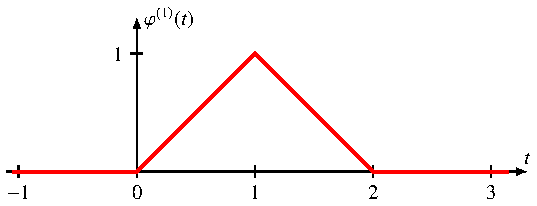
\includegraphics{chapters/9-spline/images/phi1.pdf}
\caption{Der Graph der Funktion $\varphi^{(1)}(t)$ zeigt, dass die
Funktion $\varphi^{(1)}$ stetig ist.
\label{spline:phi1}}
\end{figure}
\end{beispiel}

\begin{beispiel}
\begin{figure}
\centering
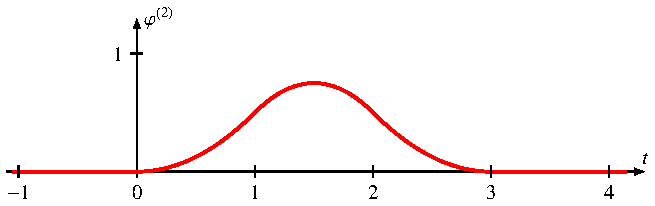
\includegraphics{chapters/9-spline/images/phi2.pdf}
\caption{Graph der Funktion $\varphi^{(2)}$
\label{spline:phi2}}
\end{figure}
Die Berechnung von $\varphi^{(2)}$ ist etwas aufwendiger.
Nach \eqref{eq:varphin-berechnung} muss
für $t\in\mathbb R$ das Integral von $\varphi^{(1)}$ über
das Interval $[t-1,t]$ berechnet werden:
\begin{align*}
&t<0:
&
\varphi^{(2)}(t)
&=0
\\
0\le\,&t<1:
&
\varphi^{(2)}(t)
&=
\int_0^t\tau\,d\tau
=
\biggl[\frac12\tau^2\biggr]_0^t = \frac12t^2
\\
1\le\,&t<2:
&
\varphi^{(2)}(t)
&=
\int_{t-1}^1 \tau\,d\tau
+
\int_1^t 2-\tau\,d\tau
=
\biggl[\frac12\tau^2\biggr]_{t-1}^1
+
\biggl[2\tau-\frac12\tau^2\biggr]_1^t
%\\
%&&
%&=
%\frac12-\frac12(t-1)^2+2t-\frac12-\frac12t^2-2+\frac12
%\\
%&&
%&=
%\frac12-\frac12t^2+t-\frac12+2t-\frac12-\frac12t^2-2+\frac12
\\
&&
&=
-t^2+3t-\frac32
=
-\biggl(t-\frac32\biggr)^2+\frac34
\\
2\le\,&t<3:
&
\varphi^{(2)}(t)
&=
\int_{t-1}^2 2-\tau\,d\tau
=
\int_0^{3-t} s\,ds
=
\frac12(3-t)^2
\\
&t>3:
&
\varphi^{(2)}(t)
&=
0
\end{align*}
Der Graph der Funktion $\varphi^{(2)}$ ist in Abbildung~\ref{spline:phi2}
dargestellt.
In Übereinstimmung mit Lemma~\ref{lemma:phidiffbar} hat die Funktion
$\varphi^{(2)}$ keine offensichtlichen ``Knickpunkte''.
\end{beispiel}

\begin{beispiel}
\begin{figure}
\centering
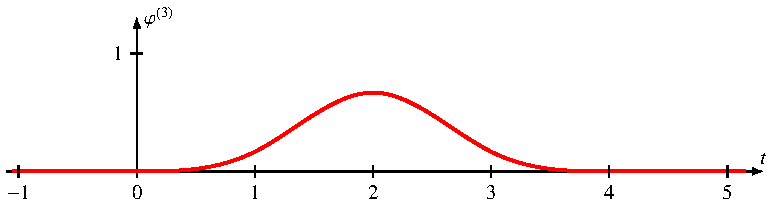
\includegraphics{chapters/9-spline/images/phi3.pdf}
\caption{Graph der Funktion $\varphi^{(3)}$.
\label{spline:phi3}}
\end{figure}
Für $\varphi^{(3)}(t)$ stellen wir nur die Resultate
zusammen, die leicht mit Hilfe eines Computer-Algebra-Systems
gewonnen werden können:
\begin{equation}
\varphi^{(3)}(t)
=
\begin{cases}
\displaystyle
\phantom{-}
\frac16t^3
&\qquad
0\le t<1
\\[9pt]
\displaystyle
-\frac12t^3+2t^2-2t+\frac23
&\qquad
1\le t<2
\\[9pt]
\displaystyle
\phantom{-}
\frac12t^3-4t^2+10t-\frac{22}3
&\qquad
2\le t<3
\\[9pt]
\displaystyle
-\frac16(t-4)^3
&\qquad
3\le t<4
\\[9pt]
\displaystyle
\phantom{-}
0&\qquad\text{sonst}
\end{cases}
\end{equation}
Der Graph der Funktion $\varphi^{(3)}$ ist in Abbildung~\ref{spline:phi3}
dargestellt.
\end{beispiel}

\subsection{Skalierungsrelation für $\varphi^{(n)}$
\label{subsection:skalierungsrelation-phin}}
Die Funktionen $\varphi^{(n)}$ können nur dann Anlass zu einer
Multiskalen-Analyse geben, wenn sie die Skalierungseigenschaft
besitzen.
Wir wissen bereits aus Abschnitt~\ref{subsection:spline:haar},
dass das Haar-Wavelet $\varphi^{(0)}$ die Skalierungsrelation
mit den Koeffizienten $1/\sqrt{2}$ erfüllt.
Satz~\ref{satz:faltung-linearkombination} garantiert, dass mit
$\varphi^{(n-1)}$ auch $\varphi^{(n)}$ die Skalierungseigenschaft hat.
Wir haben in~\eqref{eq:faltung-linearkombination}
sogar eine Formel, mit der wir die Koeffizienten der Skalierungsrelation
berechnen können.

\begin{beispiel}
Wir bestimmen die Koeffizienten der Skalierungsrelation von $\varphi^{(1)}$.
Da $\varphi^{(1)}=\varphi^{(0)}*\varphi^{(0)}$ folgt mit den bekannten
Koeffizienten $\varphi^{(0)}_0=\varphi^{(0)}_1=1/\sqrt{2}$ die
Formel~\eqref{eq:faltung-linearkombination}
\[
\begin{aligned}
\varphi^{(1)}_0
&=
\frac1{\sqrt{2}}
\varphi^{(0)}_0
\cdot
\varphi^{(0)}_0
&&=
\frac{1}{2\sqrt{2}}
=\frac{1}{2\sqrt{2}}\binom{2}{0}
\\
\varphi^{(1)}_1
&=
\frac1{\sqrt{2}}
(
\varphi^{(0)}_0
\cdot
\varphi^{(0)}_1
+
\varphi^{(0)}_1
\cdot
\varphi^{(0)}_0
)
&&=
\frac{2}{2\sqrt{2}}
=\frac{1}{2\sqrt{2}}\binom{2}{1}
\\
\varphi^{(1)}_2
&=
\frac1{\sqrt{2}}
\varphi^{(0)}_1
\cdot
\varphi^{(0)}_1
&&=
\frac{1}{2\sqrt{2}}
=\frac{1}{2\sqrt{2}}\binom{2}{2}
\end{aligned}
\]
Diese Koeffizienten haben wir im Wesentlichen schon in
\eqref{eq:skalierung-phi1-proto} angetroffen.
\end{beispiel}

Das Beispiel lässt sich verallgemeinern und führt auf den folgenden Satz.

\begin{satz}
Die Funktion $\varphi^{(n)}$ hat die Skalierungseigenschaft  mit den
Koeffizienten
\[
\varphi^{(n)}_k = \frac{1}{(\sqrt{2})^{n+2}}\binom{n}{k}.
\]
für $0\le k\le n$.
\end{satz}





%
% wavelet.tex
%
% (c) 2019 Prof Dr Andreas Müller, Hochschule Rapperswil
%
\section{Wavelets
\label{section:spline-wavelets}}
\rhead{Spline-Wavelet}
Die Funktionen $B_n$ erfüllen eine Skalierungsrelation, es besteht also
die Hoffnung, dass daraus eine Multiskalen-Analyse konstruiert werden kann.
Dazu muss zunächst die Fourier-Transformierte von $B_n$ bestimmt werden,
da alle Konstruktionen von Abschnitt~ \ref{section:skalfour} im
Frequenzbereich stattgefunden haben.
Anschliessend kann das Orthonormalisierungsverfahren von
Abschnitt~\ref{section:orthonormalisierung} auf die Funktionen $B_n$
angewendet werden.
Schliesslich kann man aus den Koeffizienten der Skalierungsrelation
auch die Koeffizienten des Wavelets ableiten und so das Wavelet
bestimmen.

\subsection{Fourier-Transformierte $\hat{B}_n$
\label{subsection:spline-ft}}
Die Fourier-Transformierte von $B_n$ kann dank der Faltungsformel für die
Fourier-Transfomierte 
\begin{equation}
\hat{B}_n = \widehat{B_0 * B_{n-1}} = \sqrt{2\pi}\hat{B}_0 \cdot \hat{B}_{n-1}
\qquad
\hat{B}_n = (\!\sqrt{2\pi})^n \hat{B}_0^{n-1}
\label{Bn-ft}
\end{equation}
berechnet werden.
Es muss also nur $\hat{B}_0$ berechnet werden.

Die Fourier-Transformierte von $B_0$ ist
\begin{align*}
\hat{B}_0(\omega)
&=
\frac1{\sqrt{2\pi}}
\int_{-\infty}^{\infty}
B_0(t) e^{-i\omega t}\,dt
=
\frac1{\sqrt{2\pi}}
\int_0^1 e^{-i\omega t}\,dt
=
\frac1{\sqrt{2\pi}}
\biggl[
\frac{1}{-i\omega} 
e^{-i\omega t}
\biggr]_0^1
\\
&=
\frac1{\sqrt{2\pi}}
\frac{e^{-i\omega}-1}{-i\omega}
=
\frac1{\sqrt{2\pi}}
\frac{1-e^{-i\omega}}{i\omega}
=
\frac1{\sqrt{2\pi}}
\frac{2}{\omega}
e^{-i\omega/2}
\frac{e^{i\omega/2} - e^{-i\omega/2}}{2i}
\\
&=
\frac1{\sqrt{2\pi}}
e^{-i\omega/2}
\frac{\displaystyle\sin\frac{\omega}2}{\displaystyle\frac{\omega}2}
=
\frac1{\sqrt{2\pi}}
e^{-i\omega/2}
\si\frac{\omega}2.
\end{align*}
Daraus und aus \eqref{Bn-ft} folgt jetzt der folgende Satz

\begin{satz}
\label{satz:Bn-ft}
Die Fourier-Transformierte von $B_n$ ist
\begin{align*}
\hat{B}_n(\omega)
&=
(\!\sqrt{2\pi})^n
\hat{B}_0(\omega)^{n+1}
=
(\!\sqrt{2\pi})^n
\biggl(
\frac{1}{\sqrt{2\pi}}
e^{-i\omega/2} \si\frac{\omega}2
\biggr)^{n+1}
=
\frac{1}{\sqrt{2\pi}}
\biggl(
e^{-i\omega/2} \si\frac{\omega}2
\biggr)^{n+1},
\\
\hat{B}_n(0)
&=
\frac{e^{-i(n+1)\omega/2}}{\sqrt{2\pi}}
.
\end{align*}
\end{satz}

\subsection{Orthonormalisierung
\label{subsection:spline-orthonormalisierung}}
In Abschnitt~\ref{section:orthonormalisierung} wurde gezeigt, wie 
erreicht werden kann, dass die Translate einer Funktion orthonormiert
sind.
Dieses Verfahren soll jetzt auf die Funktionen $B_n$ angewendet werden.
Es wurde gezeigt, dass dazu zunächst die periodisierte Funktion
\[
\Phi_n(\omega)
=
2\pi \mathcal{P}|\hat{B}_n|^2(\omega)
\]
bestimmt werden muss. 
Den Periodisierungs-Operator kann man direkt berechnen:
\begin{align}
\mathcal{P} |\hat{B}_n|^2(\omega)
&=
\sum_{l\in\mathbb Z} |\hat{B}_n(\omega + 2\pi l)|^2
=
\frac{1}{2\pi}
\sum_{l\in\mathbb Z}
\biggl|
e^{-i\omega/2 -il\pi}
\si\biggl(\frac{\omega}2+l\pi\biggr)^{n+1}
\biggr|^2
\notag
\\
&=
\frac{1}{2\pi}
\sum_{l\in\mathbb Z}
\biggl|
(-1)^l
e^{-i\omega/2}
\frac{\sin\frac{\omega}2 \cdot (-1)^l}{\frac{\omega}2 + l\pi}
\biggr|^{2n+2}
\notag
\\
&=
\frac{1}{2\pi}
\sum_{l\in\mathbb Z}
\biggl(
\frac{\sin\frac{\omega}2}{\frac{\omega}2 + l\pi}
\biggr)^{2n+2}
=
\frac{1}{2\pi}
\sin^{2n+2}\frac{\omega}2
\cdot
\sum_{l\in\mathbb Z}
\biggl(
\frac{1}{\frac{\omega}2 + l\pi}
\biggr)^{2n+2}
\notag
\\
\Rightarrow\quad
\Phi_n(\omega)
=
2\pi\mathcal{P}|\hat{B}_n|^2(\omega)
&=
\biggl|\sin\frac{\omega}2\biggr|^{2n+2}
\sum_{l\in\mathbb Z}
\frac{1}{(\omega/2 + l\pi)^{2n+2}}
.
\label{Phin:expression}
\end{align}
Die Umformung in der zweiten Zeile ist nur möglich, wenn $\omega$
kein ganzzahliges Vielfaches von $2\pi$ ist, daher ist auch
\eqref{Phin:expression} nur gültig für $\omega$, die keine ganzzahligen
Vielfachen von $2\pi$ sind.

Die Formel~\eqref{Phin:expression} funktioniert nicht mehr, wenn $\omega$
ein Vielfaches von $2\pi$ ist, da dann der Zähler verschwinden kann.
Sei also $\omega = 2\pi k$ mit $k\in\mathbb Z$.
Wir müssen die Funktion $\si$ auf den Argumenten
$\omega/2+l\pi$ auswerten.
Wegen $\omega/2 + l\pi=k\pi + l\pi = (k+l)\pi$ sind dies die ganzzahligen
Vielfachen von $\pi$, deren Sinus verschwindet.
Es gilt nämlich
\begin{align*}
\si (\pi k)
&=
\begin{cases}
\sin(k\pi)/k\pi&\qquad k\ne 0\\
\si(0)=1&\qquad k=0
\end{cases}
\\
&=
\delta_{0k}.
\end{align*}
Damit kann jetzt auch $\Phi_n(\omega)$ für ganzzahlige Vielfache von $2\pi$ 
berechnet werden:
\begin{align*}
\mathcal{P}|\hat{B}_n|^2(\omega)
&=
\mathcal{P}|\hat{B}_n|^2(2\pi k)
=
\mathcal{P}|\hat{B}_n|^2(0)
=
\sum_{l\in\mathbb Z} |\hat{B}_n(2\pi l)|^2
\\
&=
\frac1{2\pi}
\sum_{l\in\mathbb Z} |e^{-il\pi}\si(l\pi)|^{2n+2}
=
\frac1{2\pi}
\sum_{l\in\mathbb Z} \delta_{l0}
=
\frac1{2\pi}
\\
\Rightarrow\qquad
\Phi_n(\omega)
&=
\Phi_n(2\pi k)
=
\Phi_n(0)=1.
\end{align*}
Damit kann die Fourier-Transformierte $\hat{\varphi}_n(\omega)$ als
\[
\hat{\varphi}_n(\omega)
=
\frac{\hat{B}_n(\omega)}{\sqrt{\Phi_n(\omega)}}
=
\frac{1}{\sqrt{2\pi}}
\biggl(e^{-i\omega/2}\si\frac{\omega}2\biggr)^{n+1}
\]
geschrieben werden.

Als nächstes muss die Funktion $1/\sqrt{\Phi_n(\omega)}$ in eine komplexe
Fourier-Reihe entwickelt werden.
Da die Funktion $\si$ gerade ist, ist auch $\Phi_n(\omega)$ gerade.
Da $\Phi_n(\omega)$ gerade ist, muss dies auch mit einer reinen
Fourier-Kosinus-Reihe möglich sein.
Dies bedeutet, dass die Koeffizienten $c_k$ der komplexen Fourier-Reihe
von $1/\sqrt{\Phi_n(\omega)}$ reell sind und $c_k=c_{-k}$,
sie können mit 
der Formel
\begin{equation}
c_k = c_{-k}
=
\frac{1}{2\pi}
\int_{-\pi}^{\pi}
\frac{\cos(k\omega)}{\sqrt{\Phi_n(\omega)}}
\,d\omega
\label{sqrtPhincoef}
\end{equation}
berechnet werden.

Aus der Lösung von Aufgabe~\ref{aufgabe:orthonormalisierung} ist bekannt,
dass das gesuchte Wavelet mit Hilfe der Koeffizienten $c_k$ gebildet werden 
kann:
\[
\varphi_n(\omega)
=
\sum_{k\in\mathbb Z}
c_k B_n(t-k)
=
\sum_{k\in\mathbb Z}
c_k T_kB_n(t).
\]
Da die Funktionen $B_n$ stückweise Grad-$n$-polynomiell sind, ist auch
$\varphi_n(\omega)$ stückweise Grad-$n$-po\-ly\-no\-miell.

In \cite{buch:blatter} wird sogar gezeigt, dass $\sqrt{\Phi_n(\omega)}$
als Polynom in $\cos\omega$ mit rationalen Koeffizienten geschrieben
werden kann.
Wir benötigen diese Eigenschaft im Folgenden nicht und sie ist auch nicht
weiter hilfreich für die Berechnung der Koeffizienten $c_k$, die mit
Hilfe der Formel \eqref{sqrtPhincoef}
numerisch berechnet werden müssen.

\begin{table}
\centering
\begin{tabular}{|>{$}c<{$}|>{$}r<{$}||>{$}c<{$}|>{$}r<{$}|}
\hline
 k&c_k&k&c_k\\
\hline
 0& 1.291394&16&-0.000282\\
 1&-0.174099&17& 0.000564\\
 2& 0.034928&18&-0.000282\\
 3&-0.007311&19& 0.000564\\
 4& 0.001566&20&-0.000282\\
 5& 0.000118&21& 0.000564\\
 6&-0.000172&22&-0.000282\\
 7& 0.000537&23& 0.000564\\
 8&-0.000275&24&-0.000282\\
 9& 0.000562&25& 0.000564\\
10&-0.000281&26&-0.000282\\
11& 0.000564&27& 0.000564\\
12&-0.000282&28&-0.000282\\
13& 0.000564&29& 0.000564\\
14&-0.000282&30&-0.000282\\
15& 0.000564&31& 0.000564\\
\hline
\end{tabular}
\caption{Koeffizienten des Vaterwavelets für das Spline-Wavelet mit
$n=1$, also für ein stückweise lineares Wavelet.
Das zugehörige Vaterwavelet ist in Abbildung~\ref{phi1:polygonzug}
dargestellt.
\label{table:B1-koef}}
\end{table}

\begin{beispiel}
Die numerische Berechnung der Koeffizienten $c_k$ für das Spline-Wavelet 
mit $n=1$ ergibt die Koeffizienten in Tabelle~\ref{table:B1-koef}.
Da die Funktion $\varphi_n(\omega)$ stückweise linear ist, muss man nur die
Werte für ganzzahliges $\omega$ berechnen könne, dazwischen ist
$\varphi_n(\omega)$ eine lineare Funktion.
Für $B_1$ gilt aber
\begin{align*}
B_1(k)
&=
\begin{cases}
1&\qquad k=1\\
0&\qquad 1\ne k\in\mathbb Z
\end{cases}
\\
&=\delta_{1k}
\end{align*}
Für die Linearkombination $\varphi_n(k)$ gilt daher
\[
\varphi_1(k)
=
\sum_{l\in\mathbb Z} c_l B_1(k-l)
=
\sum_{k\in\mathbb Z} c_l \delta_{1,k-l}
=
c_{k-1}.
\]
Die Koeffizienten $c_k$ sind also im Wesentlichen die Funktionswerte
$\varphi_1(k)$.
Damit lässt sich der Graph von $\varphi_1$ als Polygonzug mit den Eckpunkten
$(k,c_{k-1})$ zeichnen, wie dies in Abbildung~\ref{phi1:polygonzug}
durchgeführt ist.
\begin{figure}
\centering
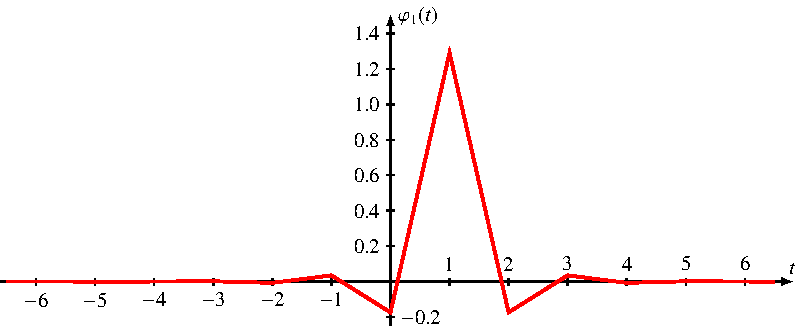
\includegraphics{chapters/9-spline/images/Bphi1.pdf}
\caption{Der Graph des stückweise linearen Vaterwavelets $\varphi_1$
ist ein Polygonzug mit den Ecken $(k,c_{k-1})$.
Die Koeffizienten $c_k$ sind in Tabelle~\ref{table:B1-koef} 
zusammengestellt.
\label{phi1:polygonzug}}
\end{figure}
\end{beispiel}

\subsection{Koeffizienten der Skalierungsrelation
\label{subsection:spline-skalierungskoeffizienten}}
Für die praktische Durchführung der Wavelet-Analyse mit Hilfe der
zugehörigen Multiskalen-Ana\-ly\-se brauchen wir die Skalierungsrelation 
für die Funktionen $\phi_n$ und daraus abgeleitet die
Skalierungsrelation für das zugehörige Wavelet $\psi_n$.

Da wir einen expliziten Ausdruck für die $\hat{\varphi}(\omega)$ haben,
können wir die Skalierungsrelation für $\varphi_n$ daraus ableiten.
Wir bezeichnen die erzeugende Funktion von $\varphi_n$ mit $H_n$.
Dann gilt
\begin{equation}
\begin{aligned}
\hat{\varphi}_n(\omega)
&=
H_n\biggl(\frac{\omega}2\biggr)
\,
\hat{\varphi}_n\biggl(\frac{\omega}2\biggr)
&&\Rightarrow&
H_n(\omega)
&=
\frac{\hat{\varphi}_n(2\omega)}{\hat{\varphi}_n(\omega)}.
\end{aligned}
\label{Hnformel}
\end{equation}
Für die Fourier-Transformierte $\hat{\varphi}_n(\omega)$ haben wir früher
\[
\hat{\varphi}_n(\omega)
=
\frac{\hat{B}_n(\omega)}{\sqrt{\Phi_n(\omega)}}
\]
erhalten.
Setzen wir dies in \eqref{Hnformel} ein, erhalten wir
\begin{equation}
H_n(\omega)
=
\frac{\hat{B}_n(2\omega)}{\hat{B}_n(\omega)}
\frac{\sqrt{\Phi_n(\omega)}}{\sqrt{\Phi_n(2\omega)}}.
\label{formel:phinskal}
\end{equation}

In Abschnitt~\ref{subsection:skalierungsrelation-phin} haben wir bereits
die Skalierungsrelation für die Spline-Funktionen $B_n$ gefunden und die
zugehörige erzeugende Funktion
\[
\tilde{H}_n(\omega) = \biggl(\frac{1+e^{-i\omega}}{2}\biggr)^{n+1}
\]
bestimmt.
Im Frequenzbereich ist die Skalierungsrelation für $\hat{B}_n(\omega)$
\[
\hat{B}_n(2\omega)=\tilde{H}_n(\omega) \, \hat{B}_n(\omega)
\qquad\Rightarrow\qquad
\frac{\hat{B}_n(2\omega)}{\hat{B}_n(\omega)}
=
\tilde{H}_n(\omega).
\]
Eingesetzt in \eqref{formel:phinskal} erhalten wir damit für die 
erzeugende Funktion 
\begin{equation}
H_n(\omega)
=
\tilde{H}_n(\omega)
\frac{\sqrt{\Phi_n(\omega)}}{\sqrt{\Phi_n(2\omega)}}
=
\biggl(
\frac{1+e^{-i\omega}}{2}
\biggr)^{n+1}
\frac{\sqrt{\Phi_n(\omega)}}{\sqrt{\Phi_n(2\omega)}}.
\label{formel:Hnf}
\end{equation}
Um die Koeffizienten von $H_n(\omega)$ zu bestimmen, müssen wir den
Bruch auf der rechten Seite in eine Fourier-Reihe entwickeln.
Da $\Phi_n(\omega)$ gerade ist, ist dies wieder mit einer Kosinus-Reihe
möglich.
Die Koeffizienten
\[
d_k
=
d_{-k}
=
\int_{-\pi}^\pi
\frac{\sqrt{\Phi_n(\omega)}}{\sqrt{\Phi_n(2\omega)}}
\,\cos(k\omega)
\,d\omega
\]
ergeben die Fourier-Reihe
\[
\frac{\sqrt{\Phi_n(\omega)}}{\sqrt{\Phi_n(2\omega)}}
=
\sum_{k\in\mathbb Z} d_k e^{ik\omega},
\]
sie müssen wie vorhin die Koeffizienten $c_k$ numerisch bestimmt werden.
Einsetzen in \eqref{formel:Hnf} liefert dann die Koeffizienten für die
erzeugende Funktion
\begin{align*}
H_n(\omega)
&=
\sum_{l=0}^{n+1} \frac1{2^{n+1}} \binom{n+1}{l} e^{-il\omega}
\cdot
\sum_{k\in\mathbb Z} d_ke^{ik\omega}
=
\sum_{l=0}^{n+1}
\sum_{k\in\mathbb Z}
\frac{1}{2^{n+1}}
\binom{n+1}{l}d_k
e^{i(k-l)\omega}
\\
&=
\sum_{s\in\mathbb Z}
e^{is\omega}
\sum_{l=0}^{n+1}
\frac{1}{2^{n+1}}
\binom{n+1}{l}d_{s-l}.
\end{align*}
Daraus liest man die Koeffizienten
\begin{equation}
h_s
= 
\sum_{l=0}^{n+1}
\frac{1}{2^{n+1}}
\binom{n+1}{l}d_{s-l}
\label{formel:hs}
\end{equation}
der Skalierungsrelation ab.

\subsection{Spline-Wavelet
\label{subsection:spline-wavelet}}
Da mit \eqref{formel:hs} die Koeffizienten der Skalierungsrelation bekannt
sind, können auch die Koeffizienten berechnet werden, mit denen das
Mutterwavelet $\psi_n$ durch die $B_n$ linear kombiniert werden kann.
In \cite{buch:blatter} ist die Berechnung der Skalierungskoeffizienten 
durchgeführt.

Die Berechnungen dieses Kapitels zeigen, dass sich für jedes $n$ ein 
stückeweise Grad-$n$-po\-ly\-no\-mi\-elles Wavelet finden lässt,
das Spline-Wavelet vom Grade $n$.
Es wird auch nach seinen Entdeckern Battle-Lemarie-Wavelet genannt.











